\documentclass{beamer}

\usepackage[utf8]{inputenc}
\usepackage{float}
\usepackage{graphicx}
\graphicspath{{./pics}}
\usepackage{comment}
\usepackage{blindtext}
\usepackage{tabularx}
\usepackage{amsmath}
\usepackage{dsfont}
\usepackage{amssymb}
\usepackage{mathtools}
\usepackage{bm}
\usepackage{textcomp}
\usepackage{anysize}
\usepackage{listings}
\usepackage{color}
\usepackage{colortbl}
\usepackage{xcolor}
\usepackage{booktabs}
\usepackage{array}
\usepackage{dcolumn}
\usepackage{longtable}
\usepackage{multirow}
\usepackage{setspace}
\usepackage{caption}
\usepackage{subcaption}
\usepackage[hidelinks]{hyperref}
\usepackage{csquotes}
\usepackage{siunitx}
\usepackage{mathabx}
\usepackage{titlesec}
\usepackage[11pt]{moresize}
\usepackage{tocloft}
\usepackage{physics}
\usepackage{enumitem}
\usepackage{slashed}
\usepackage{cancel}
\usepackage{fancyhdr}
\usepackage[backend=biber]{biblatex}
\usepackage{lmodern}
\usepackage{lipsum}
\usepackage[T1]{fontenc}

\usetheme{Madrid}
\title[QFT on a Highly Symmetric Lattice]{Quantum Field Theory on a Highly Symmetric Lattice}
%\subtitle{}
\author{Marco Aliberti}
\institute[]{Università degli Studi di Torino}
%\date{\today}
\date{\formatdate{23}{10}{2023}}

\setbeamertemplate{navigation symbols}{} % Uncomment to remove navigation buttons

\addbibresource{Bibliography.bib}

\graphicspath{{./pics}}

\newcommand{\pr}[1]{\left(#1\right)}
\newcommand{\prs}[1]{\left[#1\right]}
\newcommand{\prc}[1]{\left\{#1\right\}}
\newcommand{\C}{\mathbb{C}}
\newcommand{\R}{\mathbb{R}}
\newcommand{\Z}{\mathbb{Z}}
\newcommand{\dV}{\int\dd^4x}
\newcommand{\id}{\mathds{1}}
\newcommand{\degree}{^\circ}

\let\oldCite\cite
\renewcommand{\cite}[1]{\textsuperscript{[\oldCite{#1}]}}
\renewcommand*{\nameyeardelim}{\addcomma\space}


\begin{document}

\begin{frame}
  \titlepage
\end{frame}

\begin{frame}
  \frametitle{Why Lattice Quantum Chromodynamics?}
  \centering
  In quantum field theory scattering amplitudes in the form
  \begin{equation*}
    \bra{f}\ket{i} = \int_{\phi_i}^{\phi_f}\mathcal{D}\prs{\phi} e^{-S[\phi]}
  \end{equation*}
  need to be evaluated.
\onslide<2->
  There are two possible approaches:
  \vspace{\baselineskip}
  \begin{columns}[t]
    \column{0.5\textwidth}
    \centering
    Perturbative\\
    \vspace{\baselineskip}
    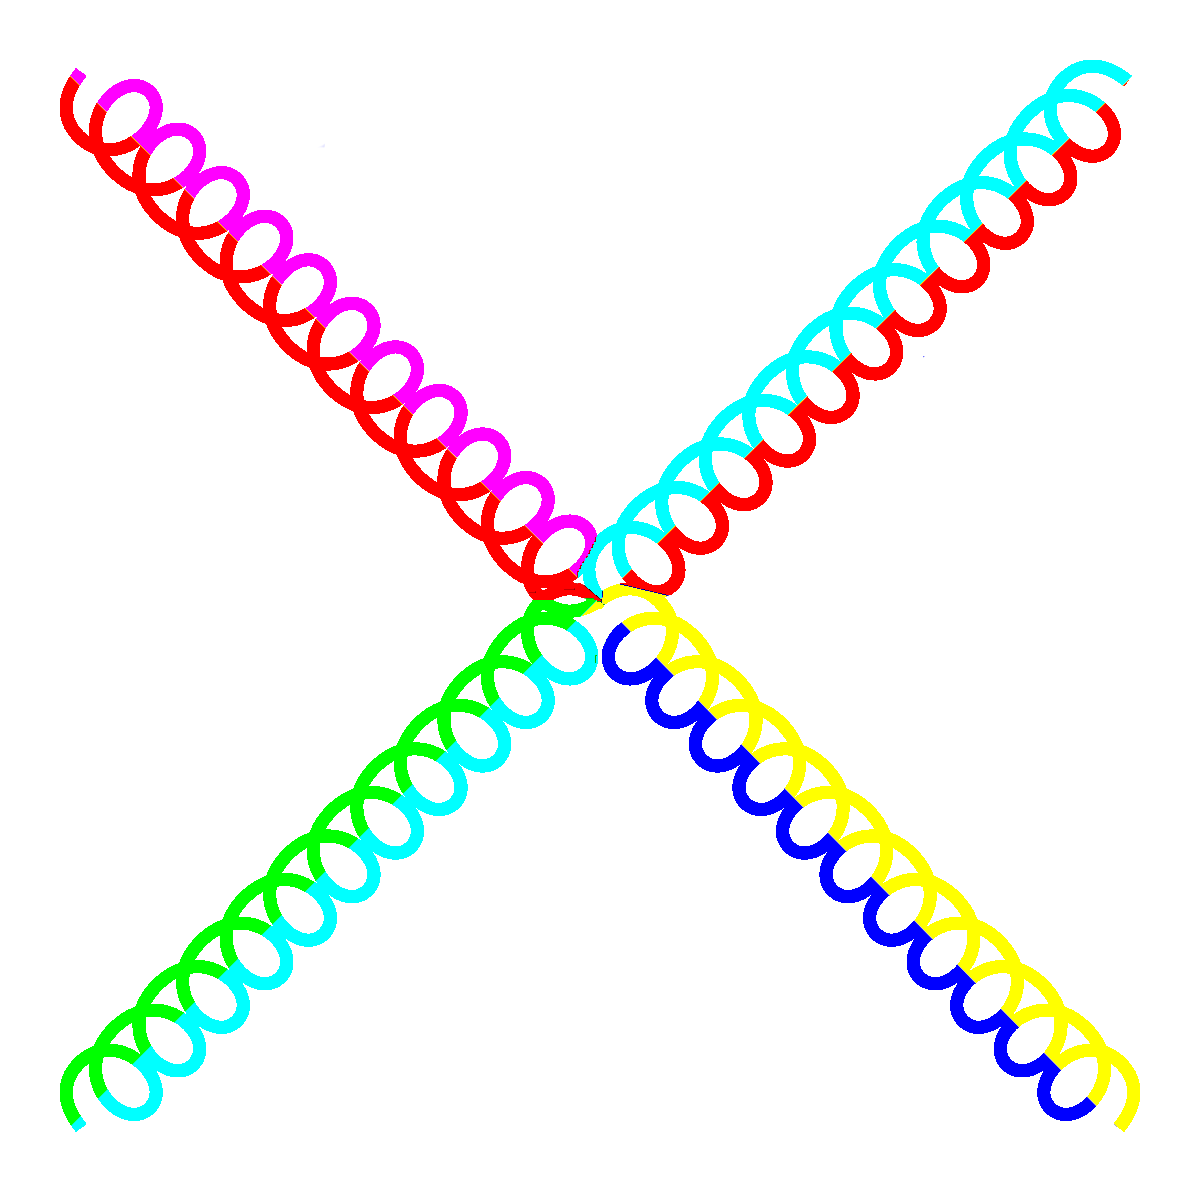
\includegraphics[width=0.4\textwidth]{gluonfd.png}
    \column{0.5\textwidth}
\onslide<3->
    \centering
    Non-Perturbative\\
    \vspace{\baselineskip}
    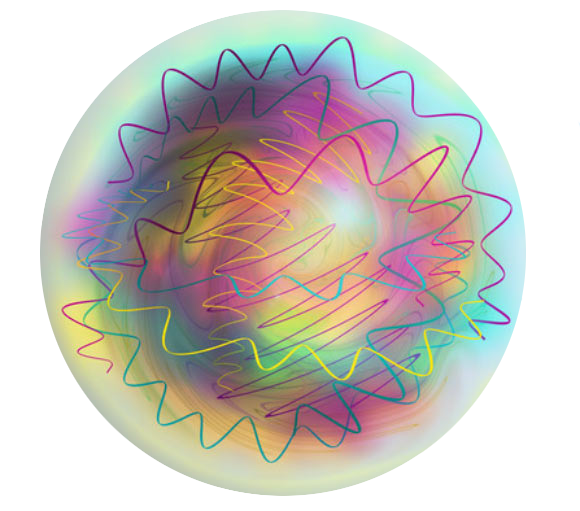
\includegraphics[width=0.45\textwidth]{Glueball.png}
  \end{columns}
\end{frame}

\begin{frame}
  \frametitle{Perturbative vs Non-Perturbative}
  \centering
  \begin{columns}[t]
    \column{0.5\textwidth}
    \centering
\onslide<1->
    Perturbative\\
    \vspace{0.5\baselineskip}
    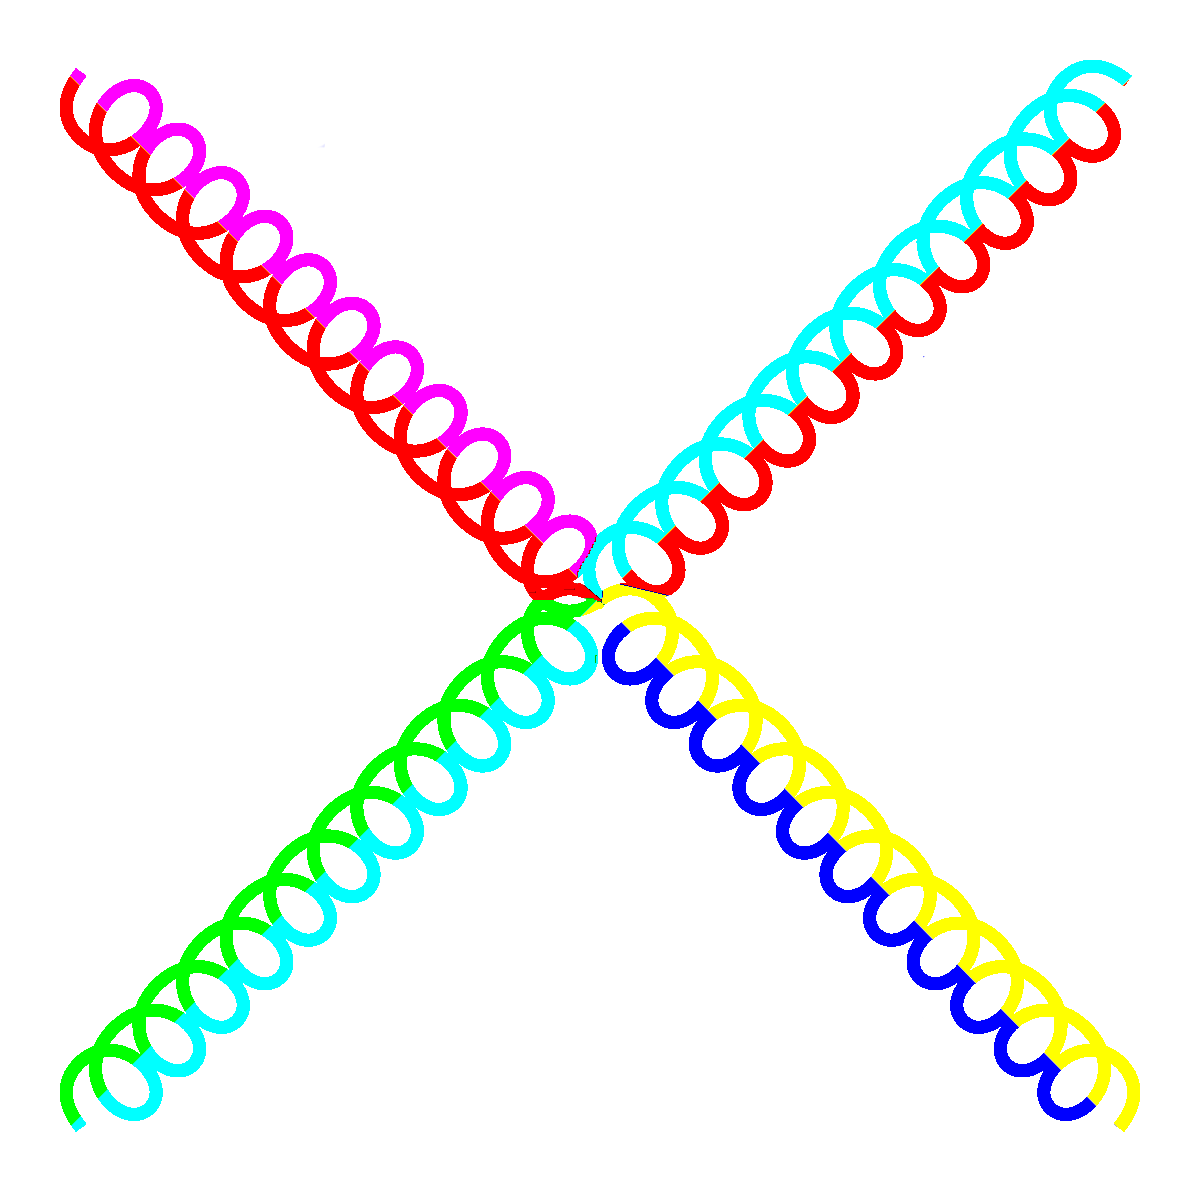
\includegraphics[height=0.4\textwidth]{gluonfd.png}\\
    \vspace{0.5\baselineskip}
    \begin{itemize}
     \item Straightforward series expansion in powers of small $g$ $\Leftrightarrow$ Feynman diagrams with $n$ loops
\onslide<2->
     \item UV divergencies need to be eliminated
\onslide<3->
     \item Fails predicting quantities with essential singularities as $g\rightarrow0$
    \end{itemize}
    \column{0.5\textwidth}
    \centering
\onslide<1->
    Non-Perturbative\\
    \vspace{0.5\baselineskip}
    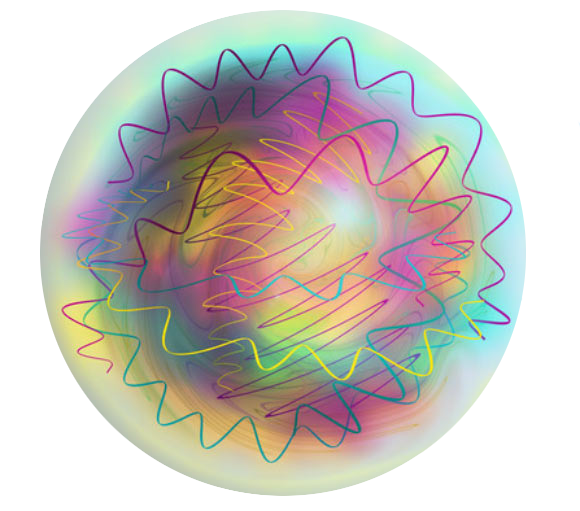
\includegraphics[height=0.4\textwidth]{Glueball.png}\\
    \vspace{0.5\baselineskip}
    \begin{itemize}
\onslide<4->
     \item No straightforward approach
\onslide<5->
     \item Can have a natural cut-off for high momenta $\Rightarrow$ No UV divergencies
\onslide<6->
     \item Can predict quantities with essential singularities as $g\rightarrow0$
    \end{itemize}
  \end{columns}
\end{frame}

\begin{frame}
  \frametitle{What is a Lattice?}
  \centering
  \begin{columns}
  \column{0.5\textwidth}
\onslide<1->
    \begin{block}{Definition: Lattice $\Lambda$}
      $\Lambda =\left\{\left.\sum _{i=1}^{n}a_{i}e_{i}\;\right\vert \;a_{i}\in \mathbb {Z} \right\}$, with $\prc{e_i}$ any basis of $\R^n$
    \end{block}
    \vspace{5\baselineskip}
\onslide<2->
    \begin{exampleblock}{Hypercubic lattice}
      $\prc{e_i}$ is the canonical basis of $\R^n$\\
      $a$ is called \emph{lattice spacing}.
    \end{exampleblock}
    \vspace{2\baselineskip}
  
  \column{0.1\textwidth}
  
  \column{0.4\textwidth}
\onslide<1->
    \centering
    \begin{figure}
      \includegraphics<1->[width=\textwidth]{two-dimensional-lattice.png}
      \caption{A bidimensional lattice.}
    \end{figure}
\onslide<2->
    \begin{figure}
      \includegraphics<1->[width=0.5\textwidth]{square-lattice.png}
      \caption{A square lattice.}
    \end{figure}
  \end{columns}
\end{frame}

\begin{frame}
  \frametitle{Lattice Field Theory}
  \centering
  \begin{columns}
  \column{0.59\textwidth}
\onslide<1->
    \begin{exampleblock}{Basic idea}
      Fields can take values only in given parts of the lattice, $x\rightarrow n\in\Lambda$.
    \end{exampleblock}
    \vspace{\baselineskip}
\onslide<2->
    Examples:
    \begin{itemize}
      \item \textcolor{blue}{Scalar fields} $\Phi(x)\rightarrow\Phi(n)$ on sites
\onslide<3->
      \item \textcolor{red}{Vector fields} $U_\mu(x)\rightarrow U_\mu(n)$ on links
\onslide<4->
      \item Object with $k$ indices on $k$-symplexes
    \end{itemize}
\onslide<5->
    \vspace{\baselineskip}
    \begin{alertblock}{Beware!}
      Spinorial fields are trickier to be discretized.
    \end{alertblock}
  
  \column{0.01\textwidth}
  
  \column{0.4\textwidth}
    \centering
\onslide<3->
    \begin{block}{Parallel Transporter}
      $U_\mu(x)=\exp(i g a A_\mu(x))$
    \end{block}
\onslide<1->
    \begin{figure}
      \includegraphics<1>[width=0.9\textwidth]{Lattice.png}
      \includegraphics<2>[width=0.9\textwidth]{LatticeScalar.png}
      \includegraphics<3->[width=0.9\textwidth]{LatticeGauge.png}\\
      \caption{A (hyper)cubic lattice in $\R^3$.}
    \end{figure}
  \end{columns}
\end{frame}

\begin{frame}
  \frametitle{Gauge-Invariant Observables and Wilson Action}
  \centering
  \vspace{0.5\baselineskip}
  \begin{columns}
  \column{0.52\textwidth}
\onslide<1->
    The Yang-Mills continuum action is $S_E=\frac14\dV F^{a\mu\nu}(x)F_{\mu\nu}^a(x)$.
\onslide<2->
    \begin{exampleblock}{Definition: Plaquette $U_{\mu\nu}(n)$}
      $U_\mu(n)U_\nu(n+\mu)U^\dagger_\mu(n+\nu)U^\dagger_\nu(n)$
    \end{exampleblock}
    
  \column{0.01\textwidth}
  \column{0.47\textwidth}
\onslide<1->
    On the lattice, every closed path is gauge-invariant.
\onslide<3->
    \begin{block}{Wilson's Idea}
      $S=\frac{\beta}{2N}\sum_{n,\mu,\nu}\mathfrak{Re}\Tr\pr{\id-U_{\mu\nu}(n)}$
    \end{block}
  \end{columns}
\onslide<1->
  \begin{figure}
    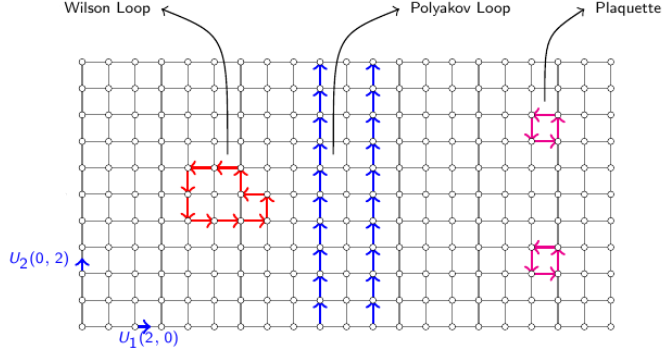
\includegraphics[height=0.4\textheight]{wilsonLoop.png}
    \caption{Gauge-invariant paths on a bidimensional lattice.\cite{SigdelDibakar2016}}
  \end{figure}
\end{frame}

\begin{frame}
  \frametitle{Polyakov Loops and Potential}
  \centering
  \vspace{0.5\baselineskip}
  \begin{columns}
  \column{0.52\textwidth}
\onslide<1->
    If the time coordinate is taken to be periodic, more closed paths arise.
    \begin{block}{Polyakov Loop}
      $P(n)=\Tr\prod_{t=0}^{T-1} U_t(n)$
    \end{block}
  
  \column{0.01\textwidth}
  \column{0.47\textwidth}
\onslide<2->
    The expectation value of two Polyakov loops is the potential.
    \begin{exampleblock}{Potential}
      $V(R)=-\frac1T\log<P(0)P^\dagger(R)>$
    \end{exampleblock}
  \end{columns}
  \vspace{0.25\baselineskip}

\onslide<1->
  \begin{figure}
    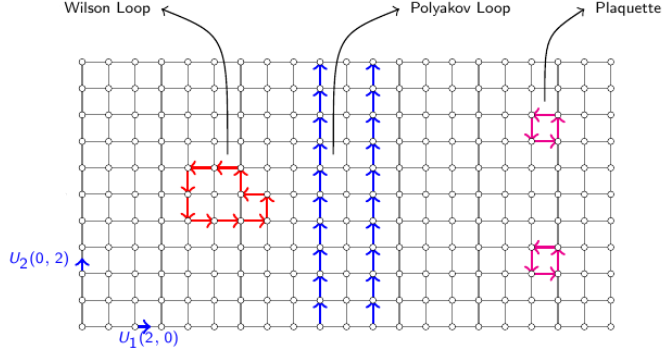
\includegraphics[height=0.4\textheight]{wilsonLoop.png}
    \caption{Gauge-invariant paths on a bidimensional lattice.\cite{SigdelDibakar2016}}
  \end{figure}
\end{frame}

\begin{frame}
  \frametitle{Lattice Symmetries}
  \centering
\onslide<1->
  Poincaré Group can be divided in:
  \begin{columns}[t]
  \column{0.45\textwidth}
    \centering
    \begin{exampleblock}{\centering Translations}
      \vspace{-\baselineskip}
\onslide<2->
      \begin{align*}
        x^\mu \rightarrow& x^\mu+\varepsilon^\mu \\
        &\Downarrow \\
        n \rightarrow& n+a\hat\mu
      \end{align*}
    \end{exampleblock}
    \vspace{2.5\baselineskip}
\onslide<4->
    $a\hat\mu \rightarrow \varepsilon^\mu$ for $a\rightarrow0$
  
  \column{0.1\textwidth}
  \column{0.45\textwidth}
    \centering
\onslide<1->
    \begin{exampleblock}{\centering Rotations}
      \vspace{-\baselineskip}
\onslide<3->
      \begin{align*}
        x^\mu \rightarrow R^\mu_\nu x^\nu &\quad R\in SO(4) \\
        &\Downarrow \\
        n \rightarrow \Gamma n &\quad \Gamma\in T
      \end{align*}
    \end{exampleblock}
    $T$: group of rotations of multiples of $90\degree$ around any axis.\\
    \vspace{0.6\baselineskip}
\onslide<5->
    $\Gamma \xcancel{\rightarrow}R$ for $a\rightarrow0$
  \end{columns}
  \vspace{\baselineskip}
  \begin{columns}
\onslide<6->
  \column{0.6\textwidth}
    \begin{alertblock}{Important:}
      Rotational invariance seems to be broken.
    \end{alertblock}
  \end{columns}
\end{frame}

\begin{frame}
  \frametitle{Rotational Invariance Restoration - Lang and Rebbi}
  Equipotential surfaces become spheres as the continuum limit is approached.
  \begin{figure}
    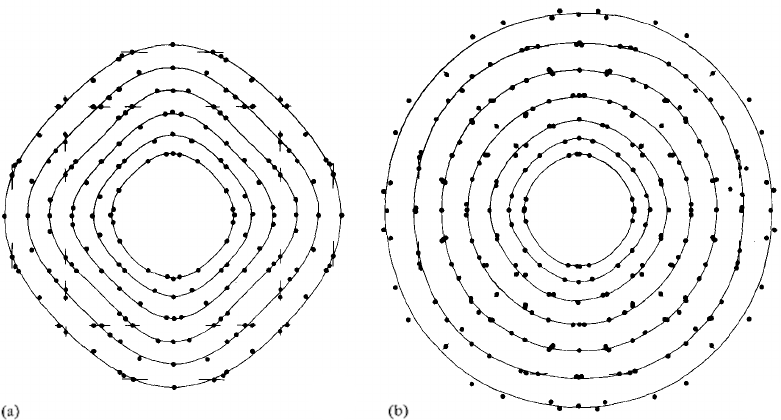
\includegraphics[width=.8\textwidth]{LangRebbi.png}
    \caption{Restoration of rotational invariance from (a) $\beta=2$, $n_s=8$, $n_t=4$ to (b)$\beta=2.25$, $n_s=16$, $n_t=6$; the curves represent equipotential curves. \cite{Lang:1982tj}}
  \end{figure}
\end{frame}

\begin{frame}
  \frametitle{Rotational Invariance Restoration}
  Values of $\beta$ are slightly different from Lang and Rebbi's because $a(\beta)\simeq\Lambda e^{-b_0\beta}$, with $\Lambda$, $b_0>0$.
  \begin{columns}
  \column{0.4\textwidth}
    \begin{figure}
      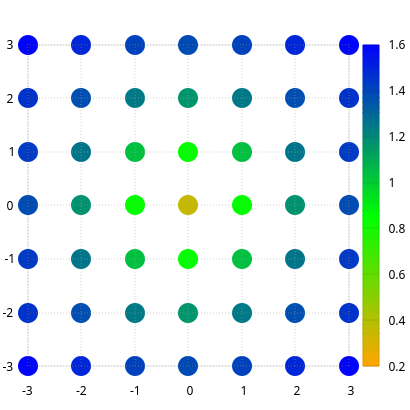
\includegraphics[width=\textwidth]{plots/XY_Plane_nt4_ns8_beta2.20_copied.png}
      \caption{Potential from $\beta=2.20$, $n_s=8$, $n_t=4$.}
    \end{figure}
  \column{0.4\textwidth}
    \begin{figure}
      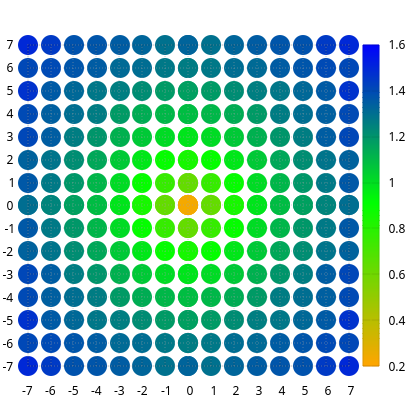
\includegraphics[width=\textwidth]{plots/XY_Plane_nt6_ns16_beta2.35_copied.png}
      \caption{Potential from $\beta=2.35$, $n_s=16$, $n_t=6$.}
    \end{figure}
  \end{columns}
\end{frame}


\begin{frame}
  \frametitle{Bibliography}
  \printbibliography
\end{frame}

\end{document}
